\begin{frame}
    \frametitle{Elementi di Codifica del testo}
    \framesubtitle{Tabella Formalismi}
    \addtocounter{nframe}{1}
    
    \begin{block}{Formalismi}
	    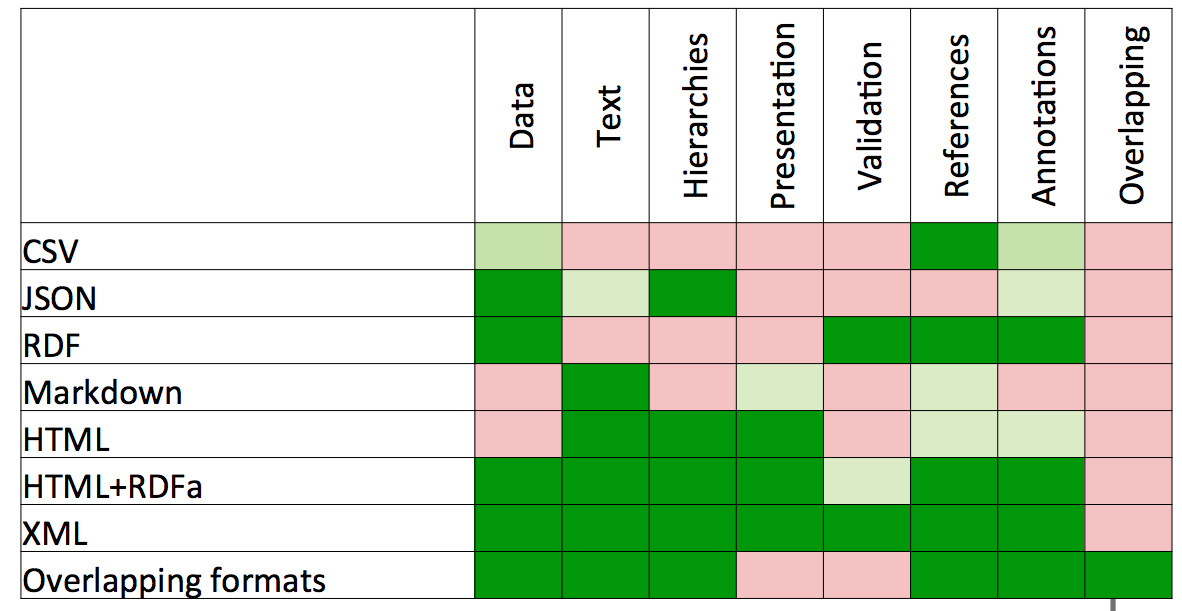
\includegraphics[width=.5\textwidth]{imgs/TabellaFormalismiCodificaTesto.png}
    \end{block}
    courtesy of \textit{Fabio Vitali}

\end{frame}


\begin{frame}
    \frametitle{Elementi di Codifica del testo}
    \framesubtitle{lista di formati}
    \addtocounter{nframe}{1}
    
    \begin{block}{Formati dato}
Data structures – CSV and tabular data
– JSON
– RDF
Plain text formats – Plain text
– TeX, LaTeX, etc.
– Markdown, CommonMark and wiki syntaxes
Markup formats
– HTML, HTML5
– XML
– HTML5+ Embedded annotations (e.g., HTML5 + RDFa)
– Markup spinoffs for overlapping (e.g. LMNL, TexMECS, etc.) 

    \end{block}

    \begin{block}{Riferimenti TEI}
        Capitolo sul character encoding e modulo Ganji 
    \end{block}

\end{frame}


% Representing text digitally 
Records
– Structures describing entities by enumerating their
properties
• Tables
– Collections of data as lists of homogeneous
records
• Trees
– Hierarchies of data and collections
• Graphs
– Networks of information structures more or less
densely intertwined 


% mia slide sulle possibili rappresentazioni del testo


% Slide Vitali
Text is hard
• Text contains relevant information, but its
structure predates digitally representable
information collections.
• It is not data. It is not a structure. It is not a
collection.
• It is not organized in records, tables, trees,
graphs. 

% altra slide Vitali
• Text has characters, including punctuation
– We all (sort of) agree on this
• Texts is ordered
– In "To be or not to be", it is important that "To be"
comes before "not to be"
• Text has structure
• Text has presentation
• Text has grammar
• Texts has semantics
• Text has variants
• Text has a lot of things that can be said about it 



% dalla slide vitali
The ecosystem of text
• Editing
• Validating
• Printing & displaying
• Transforming and converting
• Annotating
– Annotating annotations
• Searching
• ... 

% altra slide vitali
• A data format is not only what you use to
represent the data (or text) that you have to
deal with.
• An ugly format is, basically, a format for which
you have to work a lot to obtain the things you
need.
– Like putting make up on a pig to make it pretty
• It very much depends on what is the use you
plan for your data (or text). 

% slide codifica e Markup
In a sense, of course, every piece of markup added to a text represents the result of an analysis, whether human or automatic, and so it is natural to think of representing such annotations incrementally by means of markup to a digital text.